% The two forbidden sublattices of Birkhoff's distributivity theorem:
%   a lattice is distributive  ⟺  it contains NEITHER the diamond M₃ NOR the pentagon N₅ as a sublattice.
% M₃ is modular but not distributive; N₅ is not even modular.
% Render (no Ghostscript needed):  latex m3-n5.tex && dvisvgm m3-n5.dvi -o m3-n5.svg
% Tool: TikZ/PGF (diagram_language) — publication-grade mathematical typography.
\documentclass[border=8pt]{standalone}
\usepackage{tikz}
\usepackage{amssymb}
\definecolor{bot}{HTML}{E5E7EB}
\definecolor{atom}{HTML}{DBEAFE}
\definecolor{midd}{HTML}{BFDBFE}
\definecolor{top}{HTML}{93C5FD}
\definecolor{edgec}{HTML}{6B7280}
\definecolor{capt}{HTML}{374151}
\begin{document}
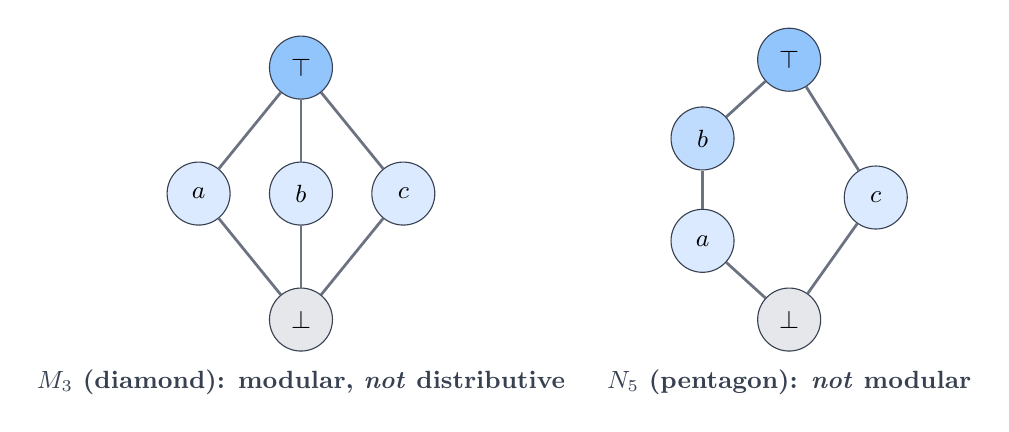
\begin{tikzpicture}[
    nd/.style={draw=capt, circle, minimum size=8mm, inner sep=1pt, fill=atom, font=\small},
    ed/.style={draw=edgec, line width=1pt},
    lbl/.style={font=\small\bfseries, text=capt}]

  % ── M₃ (diamond): ⊥, three incomparable atoms a b c, ⊤ ──
  \node[nd, fill=bot] (m0) at (0,0) {$\bot$};
  \node[nd]          (ma) at (-1.3,1.6) {$a$};
  \node[nd]          (mb) at (0,1.6)    {$b$};
  \node[nd]          (mc) at (1.3,1.6)  {$c$};
  \node[nd, fill=top](m1) at (0,3.2)    {$\top$};
  \draw[ed] (m0)--(ma); \draw[ed] (m0)--(mb); \draw[ed] (m0)--(mc);
  \draw[ed] (m1)--(ma); \draw[ed] (m1)--(mb); \draw[ed] (m1)--(mc);
  \node[lbl] at (0,-0.8) {$M_3$ (diamond): modular, \emph{not} distributive};

  % ── N₅ (pentagon): ⊥, chain a⊑b on the left, c on the right, ⊤ ──
  \begin{scope}[xshift=6.2cm]
    \node[nd, fill=bot]  (n0) at (0,0)      {$\bot$};
    \node[nd, fill=atom] (na) at (-1.1,1.0) {$a$};
    \node[nd, fill=midd] (nb) at (-1.1,2.3) {$b$};
    \node[nd, fill=atom] (nc) at (1.1,1.55) {$c$};
    \node[nd, fill=top]  (n1) at (0,3.3)    {$\top$};
    \draw[ed] (n0)--(na); \draw[ed] (na)--(nb); \draw[ed] (nb)--(n1);
    \draw[ed] (n0)--(nc); \draw[ed] (nc)--(n1);
    \node[lbl] at (0,-0.8) {$N_5$ (pentagon): \emph{not} modular};
  \end{scope}
\end{tikzpicture}
\end{document}
